\subsection{Amount of tissue}
\label{sec:amount-results}
When the concentration is known, the area scales with the amount with an error of 15--21\,\%
(Table~\ref{tab:amount}, Figure~\ref{fig:amount}). But \SI{1}{\milli\litre} of high
concentration gives 3.2 times the area of middle (dye ratio 4.8), so with one $k$ for both the
error rises to 68\,\%. A re-suction gives 0.5--0.7 times the area of the first suction.
With only four or five recordings per group, the 95\,\% prediction interval for a new recording
is wide: a factor of 1.7 above and below the line for high, 2.0 for middle and 2.2 for the tumour
(shaded in Figure~\ref{fig:amount}).

\begin{figure}[H]
  \centering
  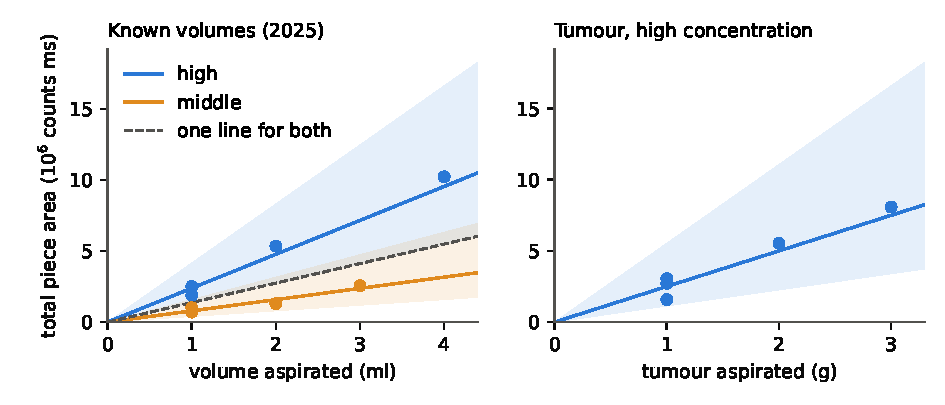
\includegraphics[width=\linewidth]{img/fig_amount.pdf}
  \caption{Total piece area of the first suction against the known amount. Lines: fitted $k$
           for each concentration; shaded: 95\,\% prediction interval for the first suction of a new recording;
           dashed: one $k$ for both.}
  \label{fig:amount}
\end{figure}

\begin{table}[H]
  \centering
  \caption{Mean error of the estimated amount (first suction, leave one recording out).
           $n$: number of recordings.}
  \label{tab:amount}
  \begin{tabular}{lrrrr}
    \toprule
    Recordings & $n$ & Count & Height\,$\times$\,width & Area \\
    \midrule
    Known volumes, high & 4 & 27\,\% & 28\,\% & 15\,\% \\
    Known volumes, middle & 4 & 46\,\% & 11\,\% & 21\,\% \\
    Tumour, high & 5 & 11\,\% & 19\,\% & 21\,\% \\
    Known volumes, concentration unknown & 8 & 32\,\% & 97\,\% & 68\,\% \\
    \bottomrule
  \end{tabular}
\end{table}

No concentration-free measure worked for both sets: area\,/\,height gave 19\,\% for the known
volumes but 46\,\% for the tumour, and the widths 31--71\,\%. Only the count was usable in both
(32\,\% and 11\,\%).

Compared with the known volumes (high), the tumour gives three times more pieces per unit amount
and half the peak height, but about the same area (\num{2.50e6} counts\,ms per gram vs
\num{2.39e6} per millilitre). The median peak width is \SI{12}{\milli\second} for the tumour and
28--\SI{30}{\milli\second} for the known volumes. At middle concentration, 10--27\,\% of the
signal above $3\sigma$ lies outside the events (high: 3--9\,\%). The threshold therefore matters
more for middle concentration: changing it from $10\sigma$ to $5\sigma$ or $20\sigma$ changes the
area of the first suction by at most 10\,\% at high concentration but by 6--23\,\% at middle
concentration (known volumes).
